\documentclass[a4paper,12pt]{article}
\usepackage[utf8]{inputenc}
\usepackage[T2A]{fontenc}
\usepackage[russian]{babel}
\usepackage{amsmath, amssymb, amsthm}
\usepackage{geometry}
\usepackage{booktabs}
\usepackage{array}
\usepackage{hyperref}
\usepackage{xcolor}
\usepackage{graphicx}
\usepackage{float}
\usepackage{caption}
\usepackage{subcaption}
% \usepackage{algorithm}
% \usepackage{algpseudocode}
\usepackage{tikz}
\usetikzlibrary{arrows.meta, positioning}

\geometry{left=2.5cm, right=2cm, top=2cm, bottom=2cm}

\hypersetup{
    colorlinks=true,
    linkcolor=blue!70!black,
    urlcolor=blue!70!black,
    citecolor=red!70!black
}

\title{Лабораторная работа №2\\Градиентный спуск: классика}
\author{Георгий Лаврентьев, Дмитрий Коваль - студенты группы М3232}
\date{10 мая 2026 г.}

\newcommand{\R}{\mathbb{R}}
\newcommand{\norm}[1]{\left\|#1\right\|}
\newcommand{\grad}{\nabla}
\newcommand{\eps}{\varepsilon}

\theoremstyle{definition}
\newtheorem{definition}{Определение}[section]
\newtheorem{theorem}{Теорема}[section]
\newtheorem{remark}{Замечание}[section]

\begin{document}
\maketitle
\vspace{-20pt}


% ═════════════════════════════════════════════════════════════
\section{Постановка задачи}
% ═════════════════════════════════════════════════════════════

Рассматривается задача безусловной минимизации:
\[
    \min_{x \in \R^n} f(x),
\]
где $f \colon \R^n \to \R$ — дифференцируемая функция.

В данной работе реализованы и исследованы четыре варианта градиентного спуска:
\begin{enumerate}
    \item градиентный спуск с постоянным шагом;
    \item градиентный спуск с дроблением шага (условие Армихо);
    \item градиентный спуск с дроблением шага (сильные условия Вольфе);
    \item метод наискорейшего градиентного спуска.
\end{enumerate}

% ═════════════════════════════════════════════════════════════
\section{Описание методов}
% ═════════════════════════════════════════════════════════════

\subsection{Общая схема методов спуска}

\begin{definition}[Общая схема метода спуска]
    Пусть выбрана начальная точка $x_0$. Будем говорить, что итерационный процесс
    $\{x_k\}_{k=0}^{\infty}$ имеет форму \emph{метода спуска}, если последовательность
    задается рекуррентным соотношением
    \[
        x_k = x_{k-1} + \beta_k u_k, \quad k \in \mathbb{N},
    \]
    где $u_k \in \mathbb{R}^n$ — единичный вектор, определяющий направление движения
    на $k$-й итерации, а $\beta_k \geq 0$ — длина шага вдоль этого направления.
\end{definition}

В данной работе в качестве направления спуска везде выбирается \textbf{антиградиент}:
\[
    u_k = -\frac{\grad f(x_{k-1})}{\norm{\grad f(x_{k-1})}}.
\]

Поэтому итерационная формула принимает вид
\begin{equation}
    \label{eq:gd_update}
    x_k = x_{k-1} - \alpha_k \grad f(x_{k-1}), \qquad k \in \mathbb{N},
\end{equation}
где $\alpha_k = \beta_k / \norm{\grad f(x_{k-1})} > 0$ — параметр шага.

Критерий остановки во всех экспериментах:
\[
    \norm{\grad f(x_k)} < \eps.
\]

\subsection{Метод 1: Постоянный шаг}

Наиболее простой вариант состоит в том, что параметр спуска фиксируется заранее и не меняется от итерации к итерации:
\[
    \alpha_k \equiv \alpha > 0.
\]
Тогда метод принимает вид
\[
    x_k = x_{k-1} - \alpha \grad f(x_{k-1}).
\]

\begin{definition}[Константа Липшица градиента]
    Функция $f$ имеет $L$-\emph{гладкий градиент}, если
    \[
        \norm{\grad f(x) - \grad f(y)} \leq L\norm{x - y}
        \quad \forall x, y \in \R^n.
    \]
\end{definition}

\begin{theorem}[Сходимость при постоянном шаге]
    Пусть $f$ выпукла и $L$-гладка. Тогда метод \eqref{eq:gd_update}
    с постоянным шагом $\alpha \in (0, 2/L)$ сходится, причём
    \[
        f(x_k) - f(x^*) \leq \frac{L\norm{x_0 - x^*}^2}{2}\cdot(1 - \alpha L)^k.
    \]
    При сильной выпуклости с константой $\mu > 0$ сходимость геометрическая.
\end{theorem}

\subsection{Метод 2: Дробление шага с условием Армихо}

Метод дробления шага не пытается решать одномерную задачу точно, но и не использует заранее фиксированный шаг без проверки. На $k$-й итерации выбирается начальное пробное значение $\alpha_0 > 0$ и коэффициент уменьшения $q \in (0,1)$. Далее проверяется некоторое условие приемлемости шага. Если оно выполнено, полагаем $\alpha_k = \alpha_0$. Если нет, шаг уменьшается: $\alpha_1 = q \alpha_0$, и проверка повторяется.

\begin{definition}[Условие Армихо]
    Для антиградиентного направления $p_k = -\grad f(x_{k-1})$ условие Армихо имеет вид
    \[
        f(x_{k-1} + \alpha p_k) \leq f(x_{k-1}) + c_1 \alpha \langle \grad f(x_{k-1}), p_k \rangle,
        \quad c_1 \in (0,1).
    \]
    Так как $p_k = -\grad f(x_{k-1})$, оно переписывается как
    \[
        f(x_k) \leq f(x_{k-1}) - c_1 \alpha_k \norm{\grad f(x_{k-1})}^2.
    \]
    Геометрически это условие означает, что новое значение функции должно уменьшиться
    достаточно заметно по сравнению с линейным прогнозом, который даёт градиент в точке $x_{k-1}$.
\end{definition}

Выбирается $\alpha_k = q^{m_k} \alpha_0$, где $m_k$ — наименьшее целое, при котором выполнено условие Армихо.
Типичные значения: $c_1 = 10^{-4}$, $q = 0.5$.

\begin{center}
\begin{tikzpicture}[scale=0.9]
    \draw[->] (-0.3,0) -- (5.5,0) node[right] {$\alpha$};
    \draw[->] (0,-0.3) -- (0,3.2) node[above] {$\phi(\alpha)$};
    \draw[blue, thick, domain=0:5, samples=100]
        plot(\x, {2.5 - 1.5*\x + 0.4*\x^2}) node[right] {$\phi(\alpha)$};
    \draw[red, dashed, domain=0:3.5]
        plot(\x, {2.5 - 0.4*\x}) node[right] {$\phi(0)-c_1\alpha\norm{g}^2$};
    \filldraw[green!60!black] (1.2, {2.5 - 1.5*1.2 + 0.4*1.2^2}) circle (3pt)
        node[above right, black] {принятый $\alpha$};
\end{tikzpicture}
\end{center}

\begin{center}
\fboxsep=10pt\relax
\fbox{
\begin{minipage}{0.8\textwidth}
\textbf{Алгоритм: Дробление шага (Армихо)}\\[10pt]
\textbf{Вход:} $x_{k-1}$, $\alpha_0 > 0$, $c_1 \in (0,1)$, $q \in (0,1)$\\
\textbf{Шаг 1:} Вычислить $g \leftarrow \grad f(x_{k-1})$, установить $\alpha \leftarrow \alpha_0$\\
\textbf{Шаг 2:} \textbf{Пока} $f(x_{k-1} - \alpha g) > f(x_{k-1}) - c_1 \alpha \norm{g}^2$:\\
\quad $\alpha \leftarrow q \cdot \alpha$\\
\textbf{Выход:} $\alpha_k = \alpha$
\end{minipage}
}
\end{center}

\subsection{Метод 3: Дробление шага с сильными условиями Вольфе}

\begin{definition}[Сильные условия Вольфе]
    Для направления $p_k = -\grad f(x_{k-1})$ сильные условия Вольфе состоят из двух неравенств:
    \begin{align}
        &\text{(Условие Армихо)} \quad
        f(x_{k-1} + \alpha p_k) \leq f(x_{k-1}) + c_1 \alpha \langle \grad f(x_{k-1}), p_k \rangle, \\
        &\text{(Условие кривизны)} \quad
        \bigl| \langle \grad f(x_{k-1} + \alpha p_k), p_k \rangle \bigr| \leq c_2 \bigl| \langle \grad f(x_{k-1}), p_k \rangle \bigr|,
    \end{align}
    где $0 < c_1 < c_2 < 1$.
\end{definition}

Для антиградиентного направления $p_k = -g_{k-1}$ эти условия принимают вид:
\begin{align}
    f(x_k) &\leq f(x_{k-1}) - c_1 \alpha_k \norm{g_{k-1}}^2, \\
    |\langle g_k, g_{k-1} \rangle| &\leq c_2 \norm{g_{k-1}}^2.
\end{align}

\begin{remark}
    Условие кривизны запрещает шаг слишком малым: требуется, чтобы $|\phi'(\alpha)|$ уменьшилось
    относительно $|\phi'(0)|$, где $\phi(\alpha) = f(x_{k-1} + \alpha p_k)$.
    Это удерживает $\alpha$ вблизи локального минимума функции $\phi(\alpha)$.

    Геометрически здесь исключаются две плохие ситуации:
    \begin{itemize}
        \item Если $\langle g_k, p_k \rangle < 0$ и по модулю всё ещё велико, то функция по-прежнему
              сильно убывает вдоль того же направления — шаг был слишком коротким.
        \item Если $\langle g_k, p_k \rangle > 0$ и по модулю велико, то производная вдоль линии
              резко сменила знак — шаг получился слишком большим.
    \end{itemize}
\end{remark}

\begin{theorem}[Существование шага Вольфе]
    Если $f$ ограничена снизу, непрерывно дифференцируема и $\langle \grad f(x_{k-1}), p_k \rangle < 0$,
    то существует $\alpha > 0$, удовлетворяющий сильным условиям Вольфе.
\end{theorem}

\subsection{Метод 4: Метод наискорейшего градиентного спуска}

\begin{definition}[Метод наискорейшего градиентного спуска]
    Методом наискорейшего градиентного спуска назовём итерационный процесс
    \[
        x_k = x_{k-1} - \alpha_k \grad f(x_{k-1}), \qquad g_{k-1} = \grad f(x_{k-1}),
    \]
    где параметр $\alpha_k$ выбирается из условия
    \[
        \alpha_k \in \arg\min_{\alpha \geq 0} f(x_{k-1} - \alpha g_{k-1}).
    \]
\end{definition}

На каждой итерации здесь возникает задача одномерной минимизации функции
\[
    \varphi_k(\alpha) = f(x_{k-1} - \alpha g_{k-1}), \qquad \alpha \geq 0.
\]

\begin{theorem}[Ортогональность соседних антиградиентов]
    Пусть функция $f(x)$ дифференцируема, а шаг $\alpha_k$ в методе наискорейшего
    градиентного спуска выбирается точным одномерным поиском. Если $g_{k-1} \neq 0$, то
    \[
        \langle g_k, g_{k-1} \rangle = 0.
    \]
\end{theorem}

\paragraph{Аналитическая формула для квадратичных функций.}
Для $f(x) = \tfrac{1}{2} x^\top A x$ ($A \succ 0$), $g_k = \grad f(x_k) = A x_k$:
\begin{equation}
    \label{eq:optimal_alpha_quad}
    \boxed{\alpha_k^* = \frac{\norm{g_k}^2}{g_k^\top A g_k}.}
\end{equation}

\begin{theorem}[Сходимость наискорейшего спуска на квадратичной функции]
    Для $f(x) = \tfrac{1}{2} x^\top A x$:
    \[
        \norm{x_k - x^*}_A \leq \left( \frac{\kappa - 1}{\kappa + 1} \right)^k \norm{x_0 - x^*}_A,
    \]
    где $\norm{\cdot}_A$ — норма, порождённая матрицей $A$. Последовательные градиенты ортогональны:
    $g_{k+1} \perp g_k$, что при большом $\kappa$ порождает зигзагообразные траектории.
\end{theorem}

% ═════════════════════════════════════════════════════════════
\section{Тестовые функции}
% ═════════════════════════════════════════════════════════════

\subsection{Квадратичные функции}

\subsubsection{\texorpdfstring{Хорошо обусловленная ($\kappa = 1$)}{Хорошо обусловленная (k=1)}}
\[
    f(x, y) = x^2 + y^2,
    \quad
    A = \begin{pmatrix} 2 & 0 \\ 0 & 2 \end{pmatrix},
    \quad \kappa(A) = 1,
    \quad x^* = (0,0).
\]
Линии уровня — концентрические окружности. Допустимый диапазон шагов: $\alpha \in (0, 1)$.

\subsubsection{\texorpdfstring{Плохо обусловленная ($\kappa = 100$)}{Плохо обусловленная (k=100)}}
\[
    g(x, y) = 50x^2 + \tfrac{1}{2}y^2,
    \quad
    A = \begin{pmatrix} 100 & 0 \\ 0 & 1 \end{pmatrix},
    \quad \kappa(A) = 100,
    \quad x^* = (0,0).
\]
Линии уровня — вытянутые эллипсы. Допустимый диапазон: $\alpha \in (0, 0.02)$.

\begin{figure}[H]
    \centering
    \begin{subfigure}[b]{0.48\textwidth}
        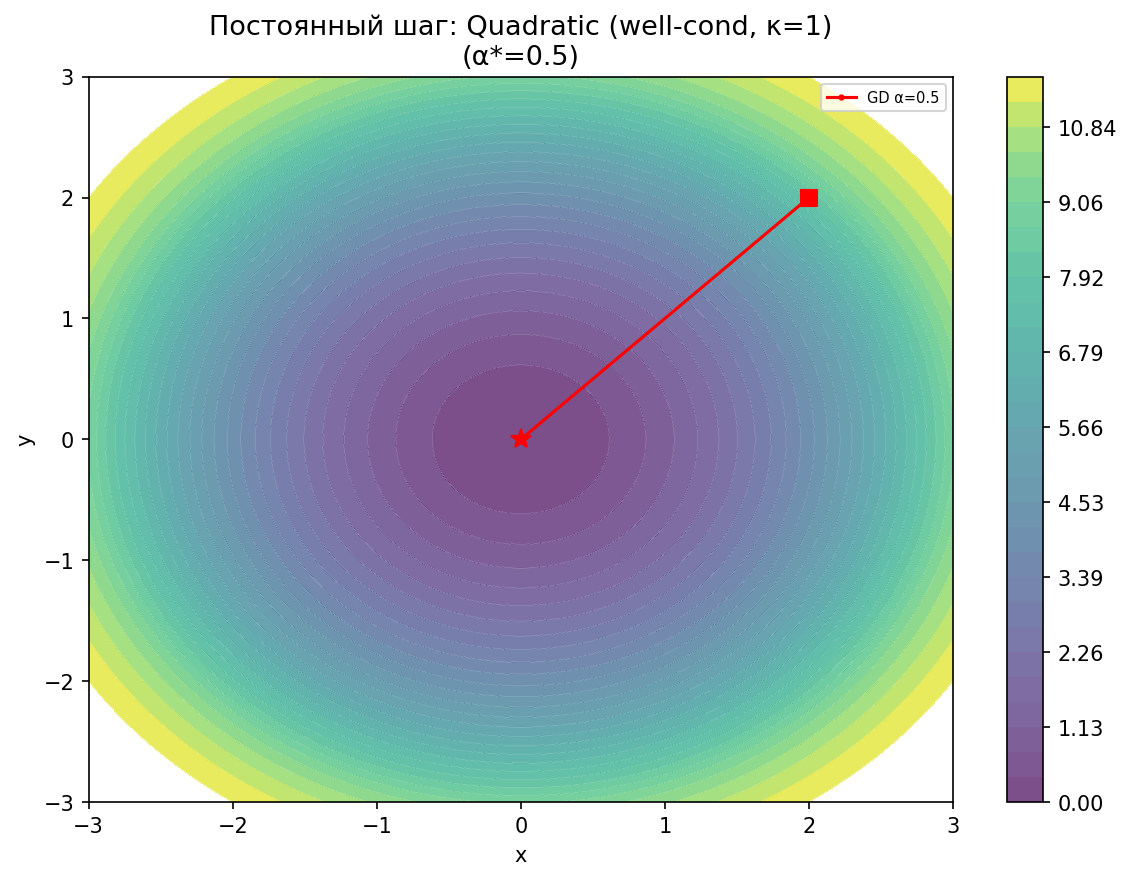
\includegraphics[width=\textwidth]{results/plots/fig_contour_const_well.png}
        \caption{Кривые уровня $f(x,y)=x^2+y^2$}
    \end{subfigure}
    \hfill
    \begin{subfigure}[b]{0.48\textwidth}
        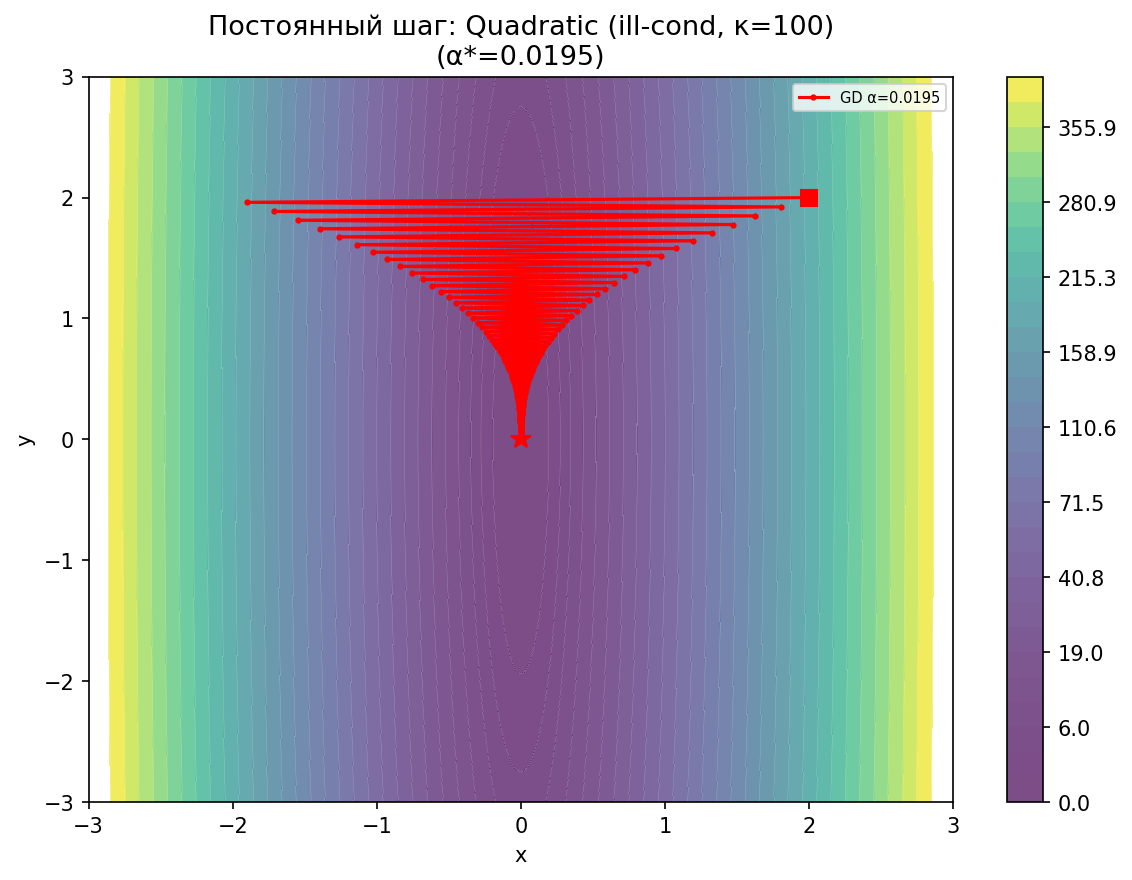
\includegraphics[width=\textwidth]{results/plots/fig_contour_const_ill.png}
        \caption{Кривые уровня $g(x,y)=50x^2+0.5y^2$}
    \end{subfigure}
    \caption{Кривые уровня квадратичных функций. Слева — сферический параболоид ($\kappa=1$),
    справа — вытянутый параболоид ($\kappa=100$).}
    \label{fig:quad_surfaces}
\end{figure}

\subsection{Функция Розенброка}
\[
    f_R(x, y) = (1 - x)^2 + 100(y - x^2)^2.
\]
Глобальный минимум: $x^* = (1, 1)$, $f_R(x^*)=0$.
Гессиан в минимуме: $\kappa(H_{f_R}(1,1)) \approx 2500$.
Функция известна своей узкой параболической долиной («бананом»).

Градиент:
\[
    \frac{\partial f_R}{\partial x} = -2(1-x) - 400x(y-x^2),
    \qquad
    \frac{\partial f_R}{\partial y} = 200(y-x^2).
\]

\begin{figure}[H]
    \centering
    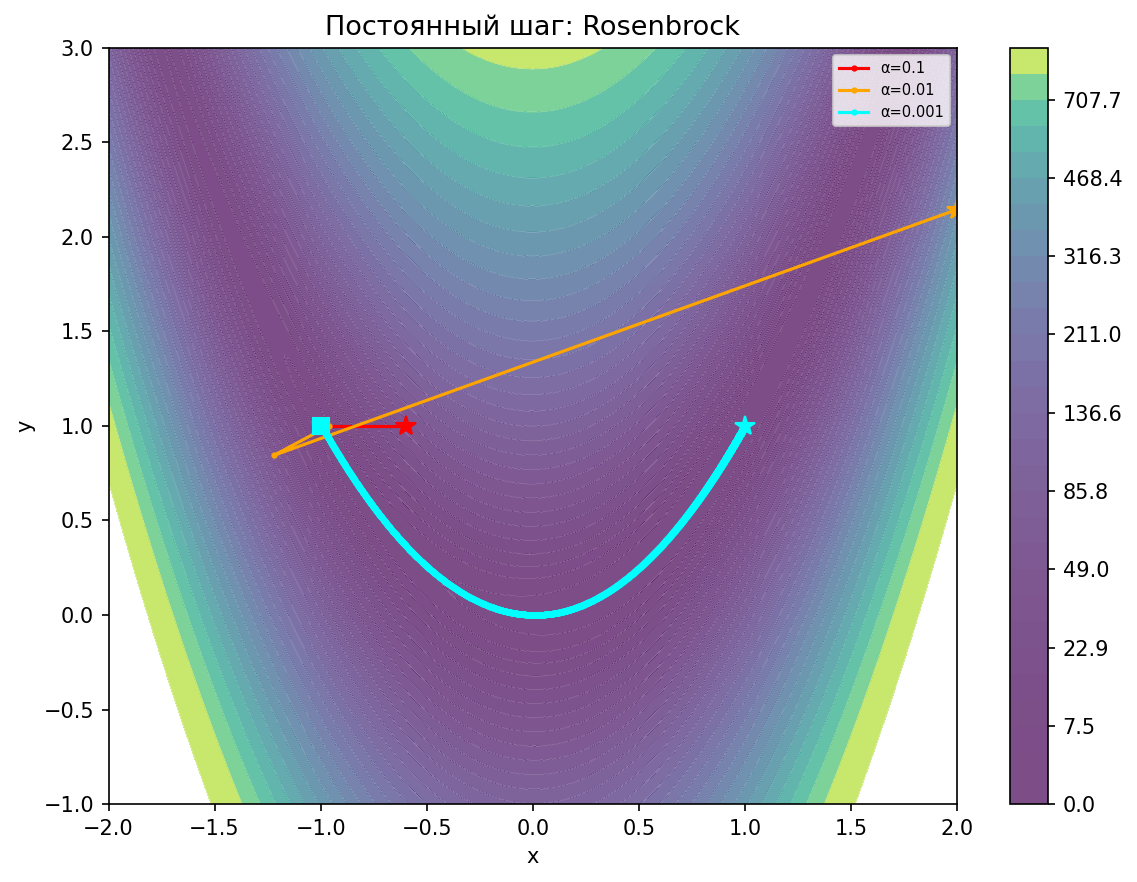
\includegraphics[width=0.55\textwidth]{results/plots/fig_contour_complex_Ros.png}
    \caption{Кривые уровня функции Розенброка. Минимум в точке $(1,1)$ находится
    на дне узкой параболической долины.}
    \label{fig:ros_surface}
\end{figure}

\subsection{Функция Экли}
\[
    f_A(x,y) = -20\exp\!\left(-0.2\sqrt{\tfrac{x^2+y^2}{2}}\right)
    -\exp\!\left(\tfrac{\cos 2\pi x + \cos 2\pi y}{2}\right) + e + 20.
\]
Глобальный минимум: $x^* = (0, 0)$, $f_A(x^*)=0$.
Многоэкстремальная: бесчисленное множество локальных минимумов на «ребристых» кольцах.

\begin{figure}[H]
    \centering
    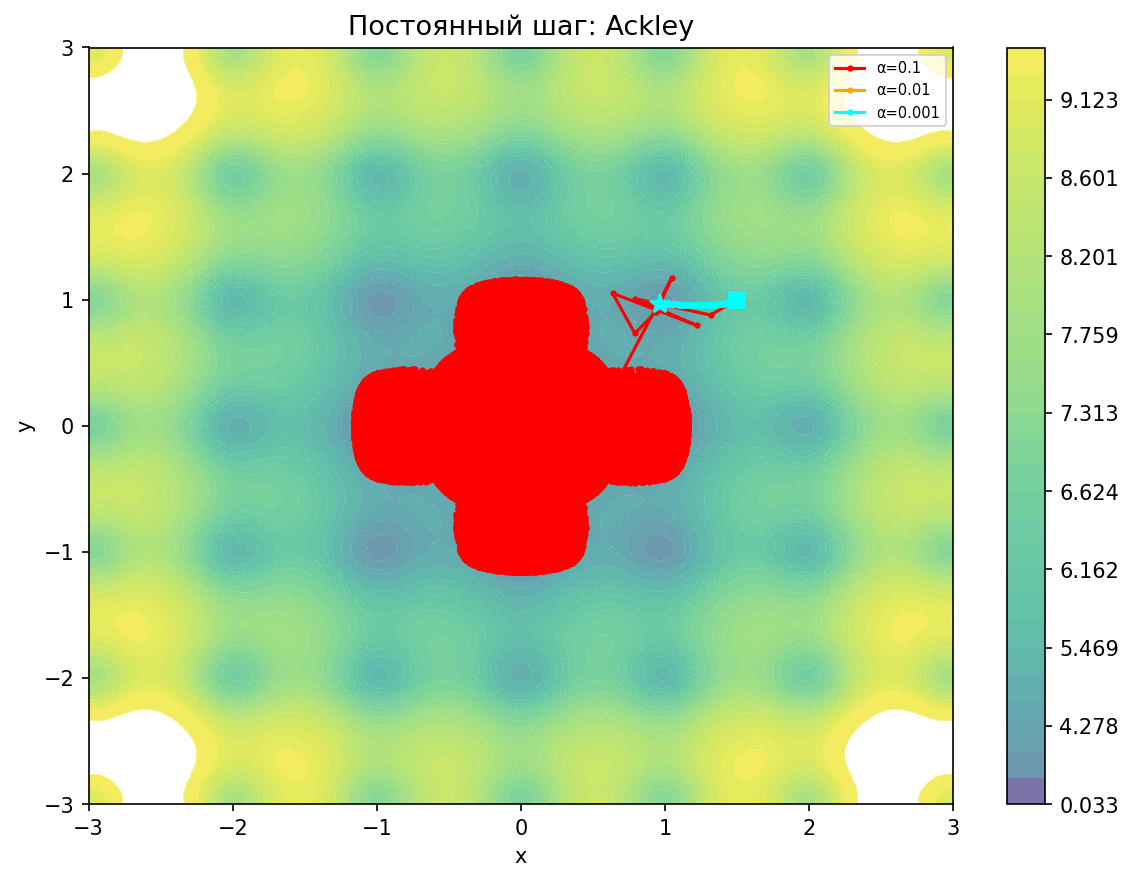
\includegraphics[width=0.55\textwidth]{results/plots/fig_contour_complex_Ack.png}
    \caption{Кривые уровня функции Экли. Хорошо видна периодическая структура
    локальных минимумов вокруг глобального минимума в начале координат.}
    \label{fig:ack_surface}
\end{figure}

\subsection{Функция Химмельблау}
\[
    f_H(x, y) = (x^2 + y - 11)^2 + (x + y^2 - 7)^2.
\]
Четыре равнозначных глобальных минимума:
$x^*_1 = (3,2)$,
$x^*_2 \approx (-2.805, 3.131)$,
$x^*_3 \approx (-3.779, -3.283)$,
$x^*_4 \approx (3.584, -1.848)$.

\begin{figure}[H]
    \centering
    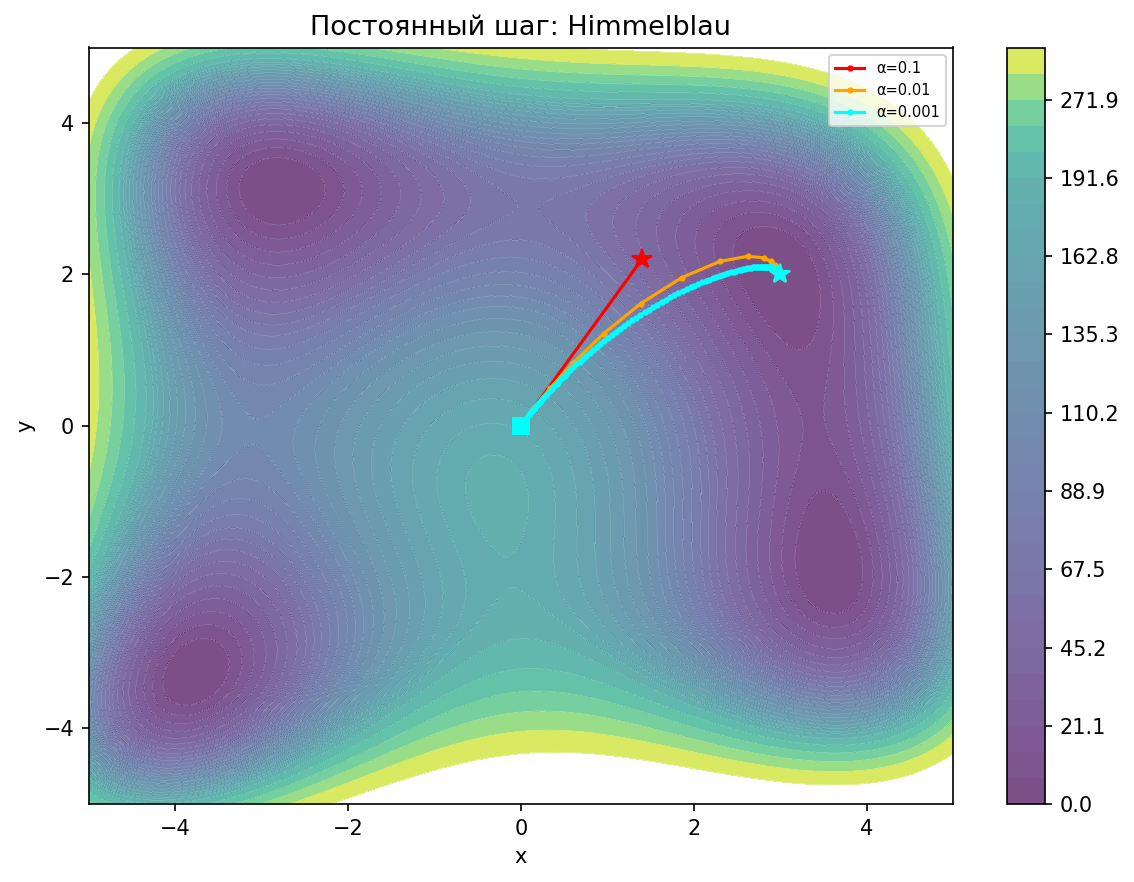
\includegraphics[width=0.55\textwidth]{results/plots/fig_contour_complex_Him.png}
    \caption{Кривые уровня функции Химмельблау. Четыре симметричных «воронки» соответствуют
    четырём глобальным минимумам функции.}
    \label{fig:him_surface}
\end{figure}

% ═════════════════════════════════════════════════════════════
\section{Экспериментальная часть}
% ═════════════════════════════════════════════════════════════

% ─────────────────────────────────────────────────────────────
\subsection{Задание 1: Постоянный шаг на квадратичных функциях}
% ─────────────────────────────────────────────────────────────

Критерий остановки: $\norm{\grad f(x_k)} < 10^{-8}$.
Стартовая точка: $x_0 = (2, 2)^\top$.

\subsubsection{Хорошо обусловленная функция ($\kappa = 1$)}

% Auto-generated table for constant-step (well-conditioned quadratic)
\input{results/tables/Quadratic__well_cond__κ_1_.tex}

\paragraph{Вывод.} Оптимальный шаг $\alpha^* = \frac{2}{\lambda_{\min}+\lambda_{\max}} = \frac{2}{2+2} = 0.5$
обеспечивает сходимость за 1 итерацию — метод попадает в минимум точно.
График числа итераций от шага имеет U-образную форму с минимумом в $\alpha=0.5$.

\begin{figure}[H]
    \centering
    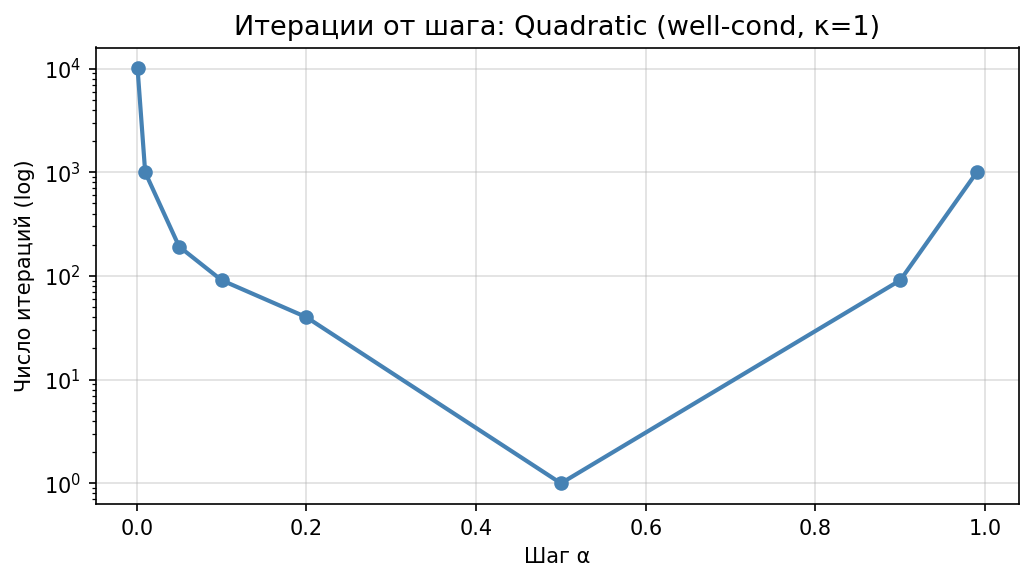
\includegraphics[width=0.65\textwidth]{results/plots/fig_iter_vs_step_well.png}
    \caption{Зависимость числа итераций от шага $\alpha$ для хорошо обусловленной
    квадратичной функции. Минимум в точке $\alpha^*=0.5$.}
    \label{fig:iter_step_well}
\end{figure}

\begin{figure}[H]
    \centering
    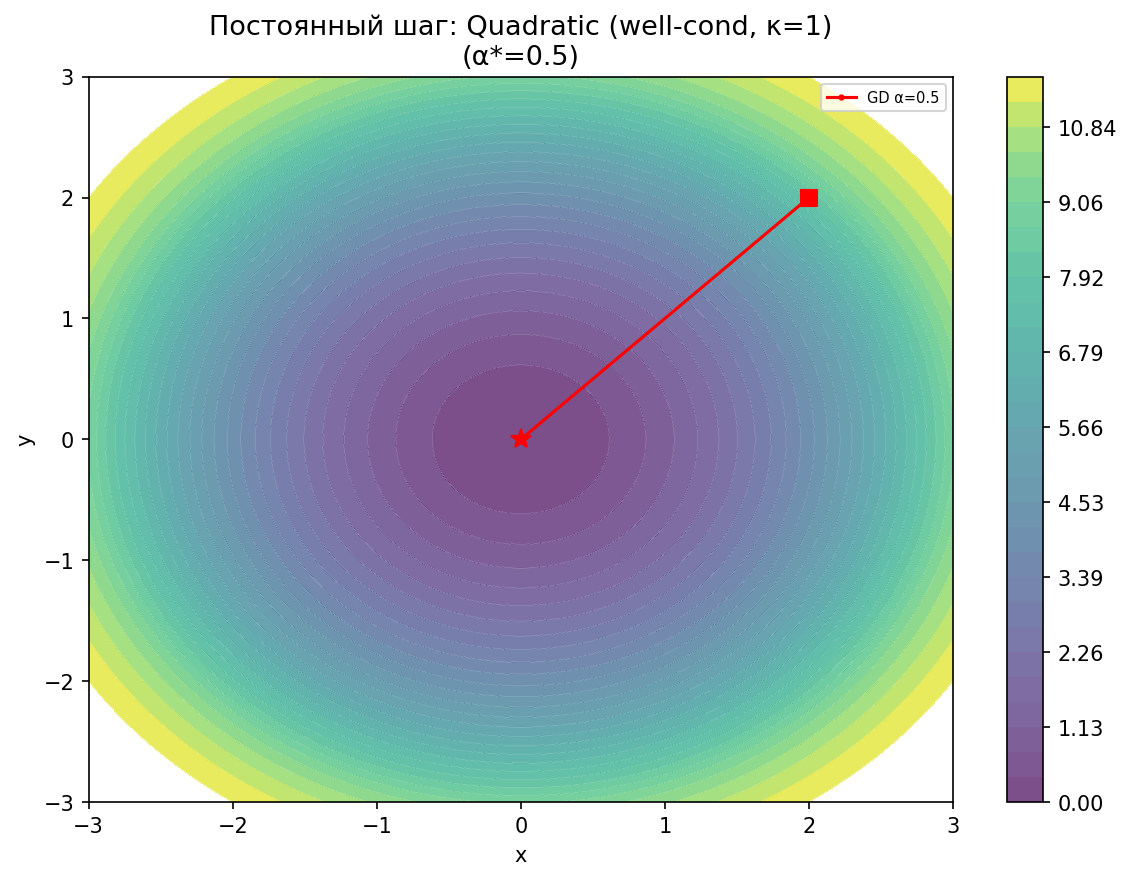
\includegraphics[width=0.65\textwidth]{results/plots/fig_contour_const_well.png}
    \caption{Траектория постоянного шага ($\alpha^*=0.5$) на линиях уровня
    $f(x,y)=x^2+y^2$. Квадрат — стартовая точка, звезда — найденный минимум.
    При $\kappa=1$ метод сходится за одну итерацию.}
    \label{fig:contour_well}
\end{figure}

\subsubsection{Плохо обусловленная функция ($\kappa = 100$)}

% Auto-generated table for constant-step (ill-conditioned quadratic)
\input{results/tables/Quadratic__ill_cond__κ_100_.tex}

\paragraph{Вывод.} Оптимальный шаг вблизи $\alpha^* = \frac{2}{100+1} \approx 0.0198$.
При $\alpha=0.0199$ (вблизи границы устойчивости $2/L=0.02$) итераций больше, чем при
$\alpha=0.0195$: метод начинает осциллировать вдоль оси $x$.
При $\alpha=0.0001$ метод не успевает сойтись за 100\,000 итераций.

\begin{figure}[H]
    \centering
    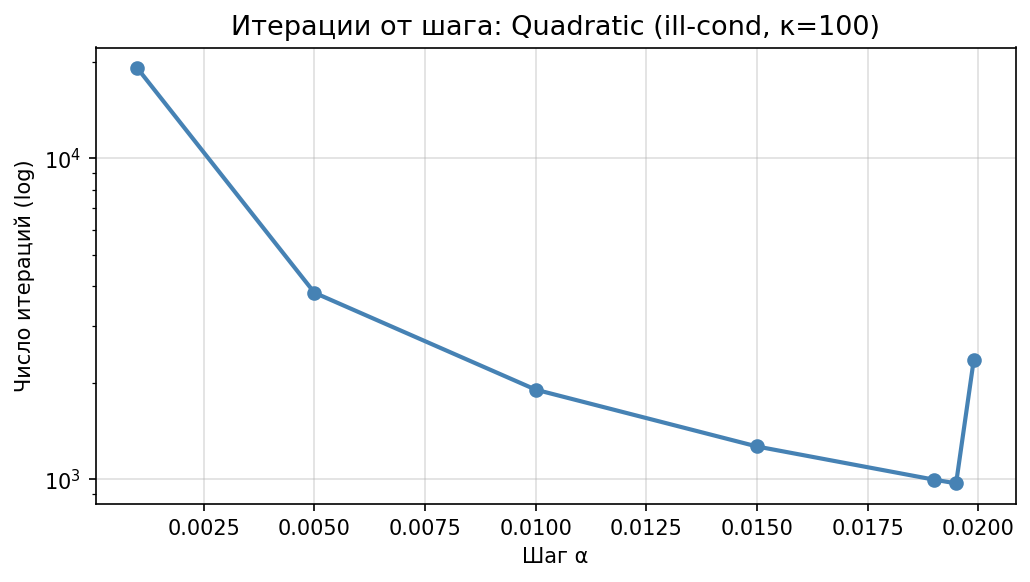
\includegraphics[width=0.65\textwidth]{results/plots/fig_iter_vs_step_ill.png}
    \caption{Зависимость числа итераций от шага $\alpha$ для плохо обусловленной
    квадратичной функции. Минимум вблизи $\alpha^* \approx 0.0195$,
    рост справа объясняется близостью к границе устойчивости.}
    \label{fig:iter_step_ill}
\end{figure}

\begin{figure}[H]
    \centering
    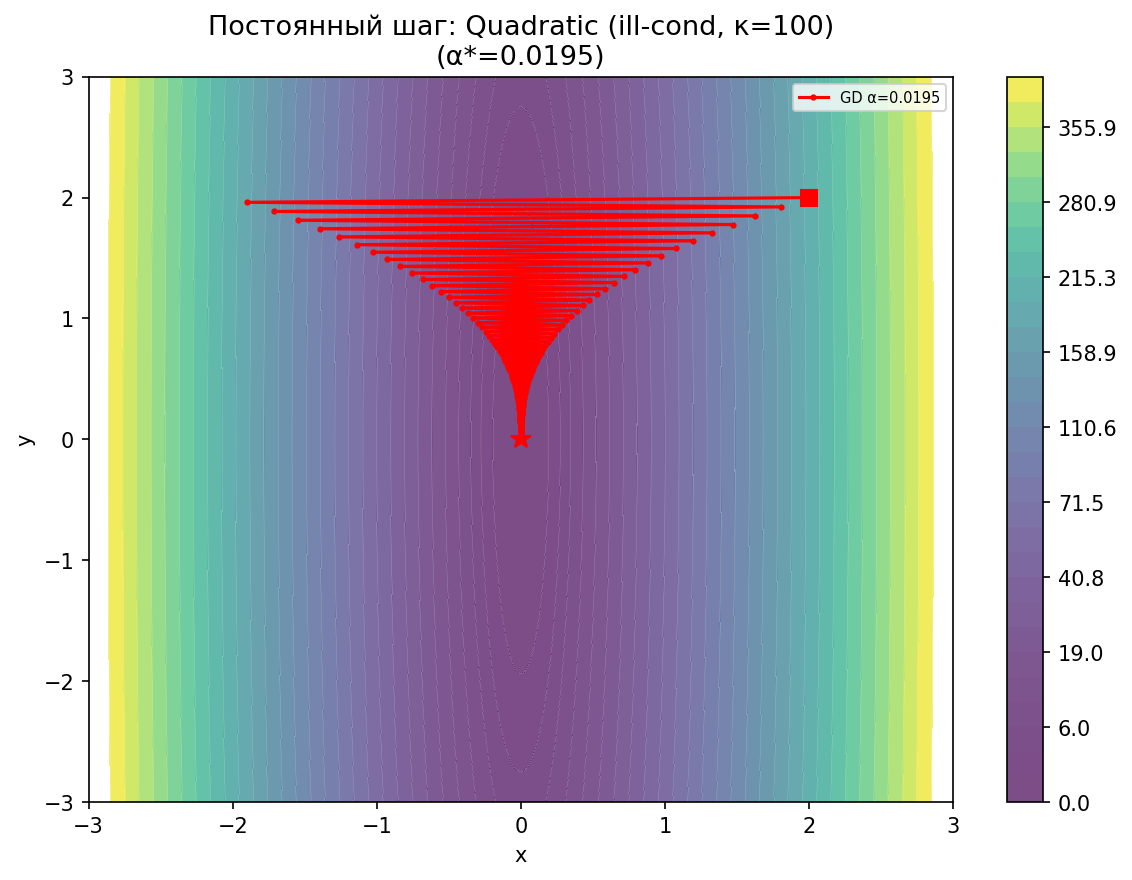
\includegraphics[width=0.65\textwidth]{results/plots/fig_contour_const_ill.png}
    \caption{Траектория постоянного шага ($\alpha^*=0.0195$) на линиях уровня
    $g(x,y)=50x^2+0.5y^2$. Видна характерная зигзагообразная траектория:
    метод чередует большие шаги вдоль оси $y$ и маленькие вдоль оси $x$.}
    \label{fig:contour_ill}
\end{figure}

% ─────────────────────────────────────────────────────────────
\subsection{Задание 2: Постоянный шаг на сложных функциях}
% ─────────────────────────────────────────────────────────────

Стартовые точки: Розенброк $(-1,1)$, Экли $(1.5,1)$, Химмельблау $(0,0)$.

\begin{table}[H]
\centering
\caption{Постоянный шаг на сложных функциях, $\eps=10^{-8}$.}
\label{tab:complex_const}
\begin{tabular}{lccccl}
\toprule
Функция & $\alpha$ & Итерации & $f(x^*)$ & $x^*$ & Сошлось? \\
\midrule
Розенброк & 0.100 & — (inf) & $\infty$ & diverged & $\times$ \\
Розенброк & 0.010 & — (inf) & $\infty$ & diverged & $\times$ \\
Розенброк & \textbf{0.001} & \textbf{43564} & $1.25\times10^{-16}$ & $(1.0000,1.0000)$ & \checkmark \\
\midrule
Экли & 0.100 & — (локал.) & 3.72 & $(-0.33, 0.44)$ & $\times$ \\
Экли & \textbf{0.010} & \textbf{39} & 3.57 & $(0.97, 0.97)$ & \checkmark \\
Экли & \textbf{0.001} & \textbf{480} & 3.57 & $(0.97, 0.97)$ & \checkmark \\
\midrule
Химмельблау & 0.100 & — (inf) & $\infty$ & diverged & $\times$ \\
Химмельблау & \textbf{0.010} & \textbf{77} & $1.94\times10^{-18}$ & $(3.0000,2.0000)$ & \checkmark \\
Химмельблау & \textbf{0.001} & \textbf{849} & $1.89\times10^{-18}$ & $(3.0000,2.0000)$ & \checkmark \\
\bottomrule
\end{tabular}
\end{table}

\paragraph{Комментарий к результатам.}
\begin{itemize}
    \item \textbf{Розенброк, $\alpha \geq 0.01$:} расходимость (inf/nan).
    Градиент вблизи стартовой точки достигает значений $\sim 400$, поэтому
    шаг $0.01$ даёт смещение $\sim 4$, откуда градиент ещё больше — и так до $\infty$.
    Только $\alpha=0.001$ достаточно мал.
    \item \textbf{Экли, $\alpha=0.1$:} метод остановился в локальном минимуме
    ($f \approx 3.72 \neq 0$) — функция многоэкстремальна, критерий $\norm{\grad f}<\eps$
    выполнился в нужной точке стационарности.
    Экли при $\alpha \in \{0.01, 0.001\}$ тоже находит \emph{локальный} минимум
    вблизи $(0.97, 0.97)$, не глобальный $(0,0)$.
    \item \textbf{Химмельблау, $\alpha=0.1$:} аналогично Розенброку — взрыв градиента.
\end{itemize}

\begin{figure}[H]
    \centering
    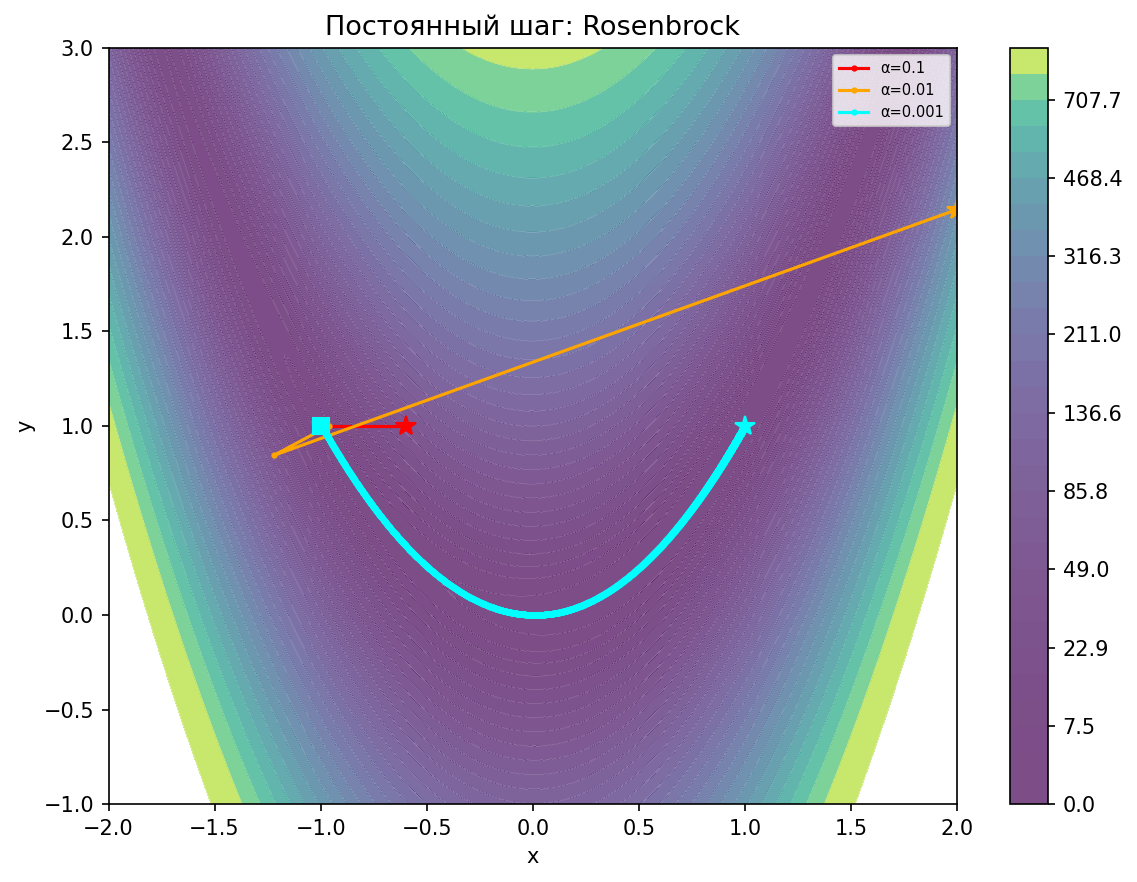
\includegraphics[width=0.75\textwidth]{results/plots/fig_contour_complex_Ros.png}
    \caption{Постоянный шаг на функции Розенброка.
    $\alpha=0.1$ и $\alpha=0.01$ — расходимость.
    $\alpha=0.001$ (голубой) — медленная сходимость вдоль параболической долины.}
    \label{fig:complex_ros}
\end{figure}

\begin{figure}[H]
    \centering
    \begin{subfigure}[b]{0.48\textwidth}
        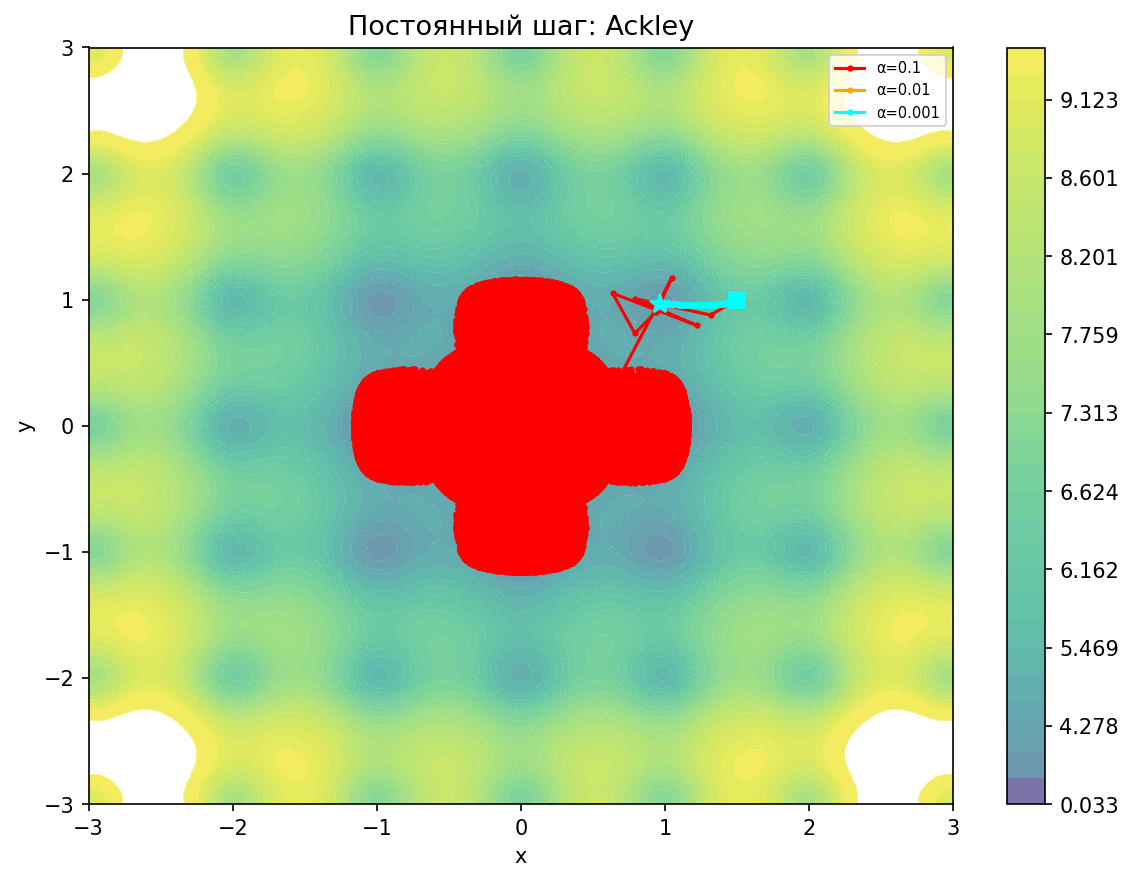
\includegraphics[width=\textwidth]{results/plots/fig_contour_complex_Ack.png}
        \caption{Функция Экли}
    \end{subfigure}
    \hfill
    \begin{subfigure}[b]{0.48\textwidth}
        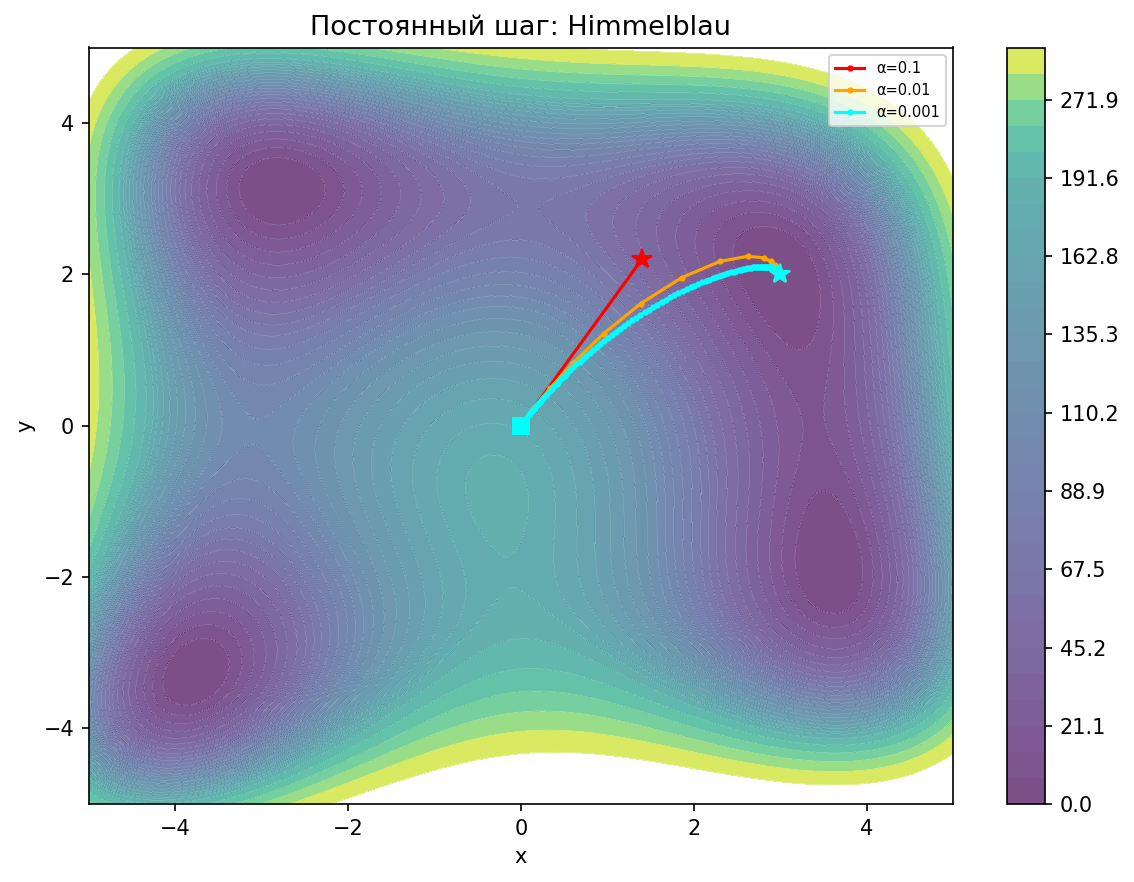
\includegraphics[width=\textwidth]{results/plots/fig_contour_complex_Him.png}
        \caption{Функция Химмельблау}
    \end{subfigure}
    \caption{Постоянный шаг на многоэкстремальных функциях.
    Экли: большой шаг ($\alpha=0.1$) прыгает между ребристыми кольцами.
    Химмельблау: $\alpha=0.01$ и $0.001$ сходятся к одному из четырёх минимумов.}
    \label{fig:complex_ack_him}
\end{figure}

% ─────────────────────────────────────────────────────────────
\subsection{Задание 4: Методы дробления шага — зависимость от точности}
% ─────────────────────────────────────────────────────────────

Исследуется зависимость числа итераций, вызовов $f$ и $\grad f$ от
$\varepsilon \in \{10^{-1}, \ldots, 10^{-8}\}$, $x_0=(2,2)$.

\subsubsection{Хорошо обусловленная квадратика ($\kappa=1$)}

% Table(s) generated automatically from CSV; include the LaTeX fragments
\input{results/tables/Quadratic__well_cond__κ_1____Армихо.tex}
\input{results/tables/Quadratic__well_cond__κ_1____Вольфе.tex}

\paragraph{Вывод.} Оба метода находят точный минимум за \textbf{1 итерацию}
независимо от $\varepsilon$. Линейный поиск выбирает шаг $\alpha=0.5$ — точный
оптимум для данной сферической квадратики.

\subsubsection{Плохо обусловленная квадратика ($\kappa=100$)}

% Table(s) generated automatically from CSV; include the LaTeX fragments
\input{results/tables/Quadratic__ill_cond__κ_100____Армихо.tex}
\input{results/tables/Quadratic__ill_cond__κ_100____Вольфе.tex}

\paragraph{Вывод.} На плохо обусловленной квадратике при строгой точности оба метода требуют большого числа итераций (для примера, при $\eps=10^{-8}$ число итераций порядка нескольких сотен). Вольфе даёт схожие по качеству результаты со слегка иным профилем вычислений: условие кривизны требует вычисления градиента в пробных точках, поэтому в таблице видно, что число вызовов $\nabla f$ у Вольфе сопоставимо с числом вызовов $f$. При практическом применении это означает компромисс между более «устойчивым» выбором шага и увеличенной стоимостью вычисления градиентов.

\begin{figure}[H]
    \centering
    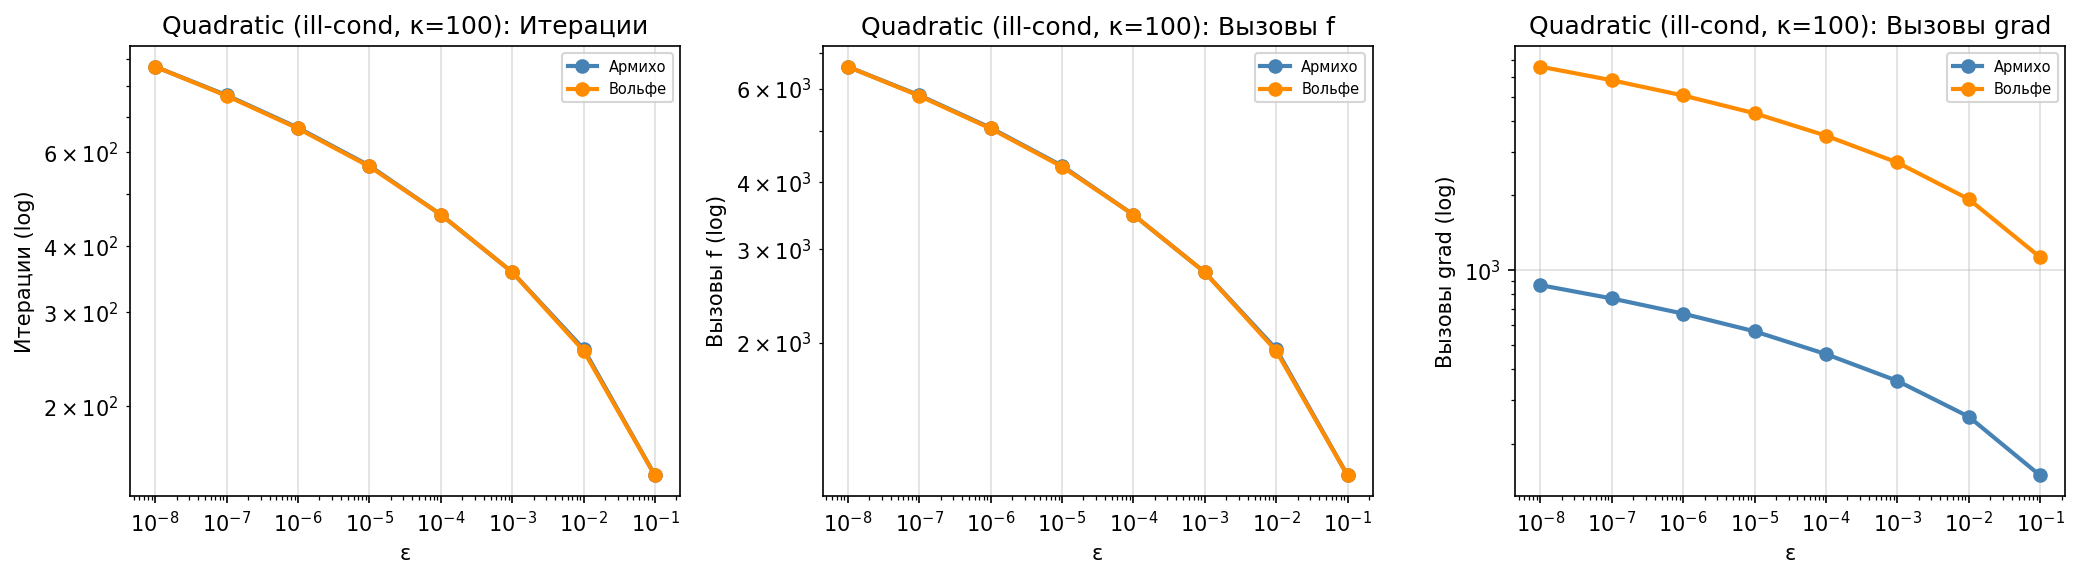
\includegraphics[width=\textwidth]{results/plots/fig_eps_ill.png}
    \caption{Зависимость числа итераций, вызовов $f$ и $\grad f$ от точности $\eps$
    для плохо обусловленной квадратики. Армихо (синий): линейный рост числа итераций;
    Вольфе (оранжевый): схожая зависимость по числу итераций, но поиск шага в Вольфе
    требует большого числа вычислений градиента (см. столбцы "вызовы $\nabla f$").}
    \label{fig:eps_ill}
\end{figure}

\begin{figure}[H]
    \centering
    \begin{subfigure}[b]{0.48\textwidth}
        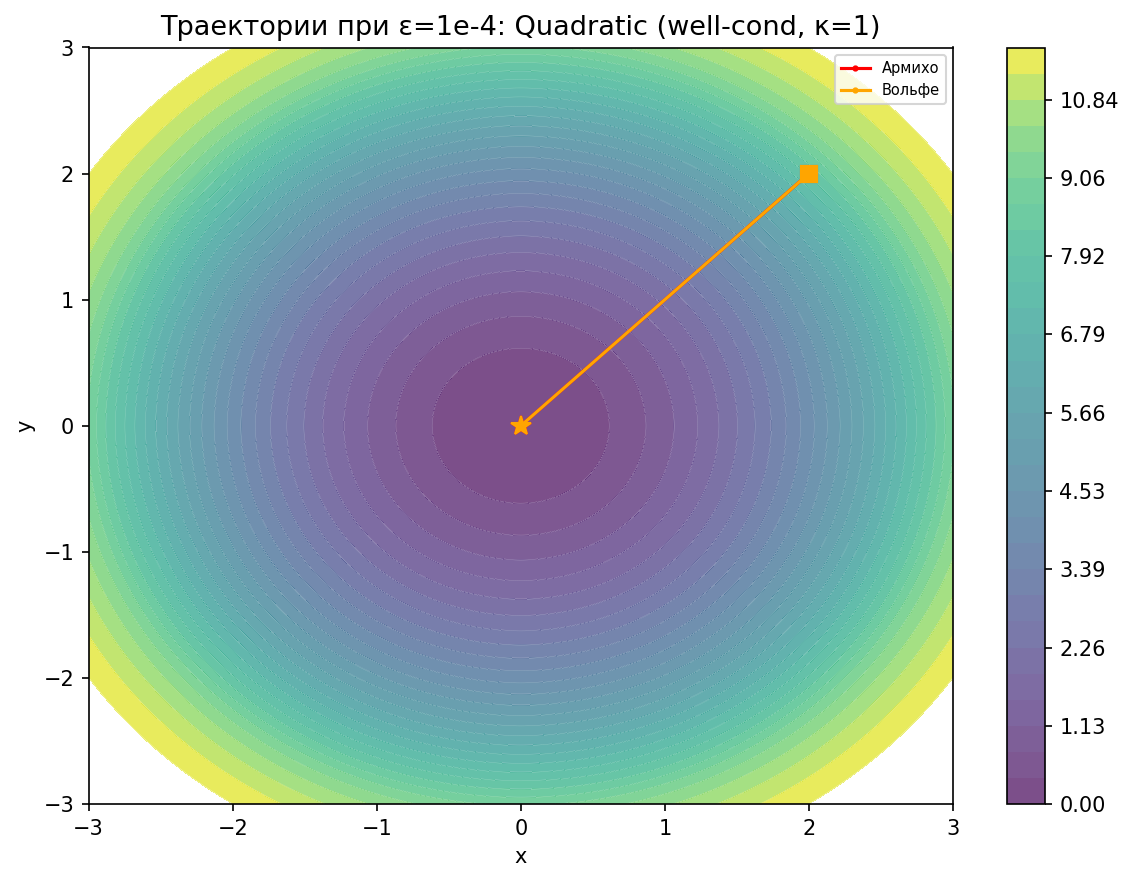
\includegraphics[width=\textwidth]{results/plots/fig_traj_linesearch_well.png}
        \caption{Хорошо обусловленная ($\kappa=1$)}
    \end{subfigure}
    \hfill
    \begin{subfigure}[b]{0.48\textwidth}
        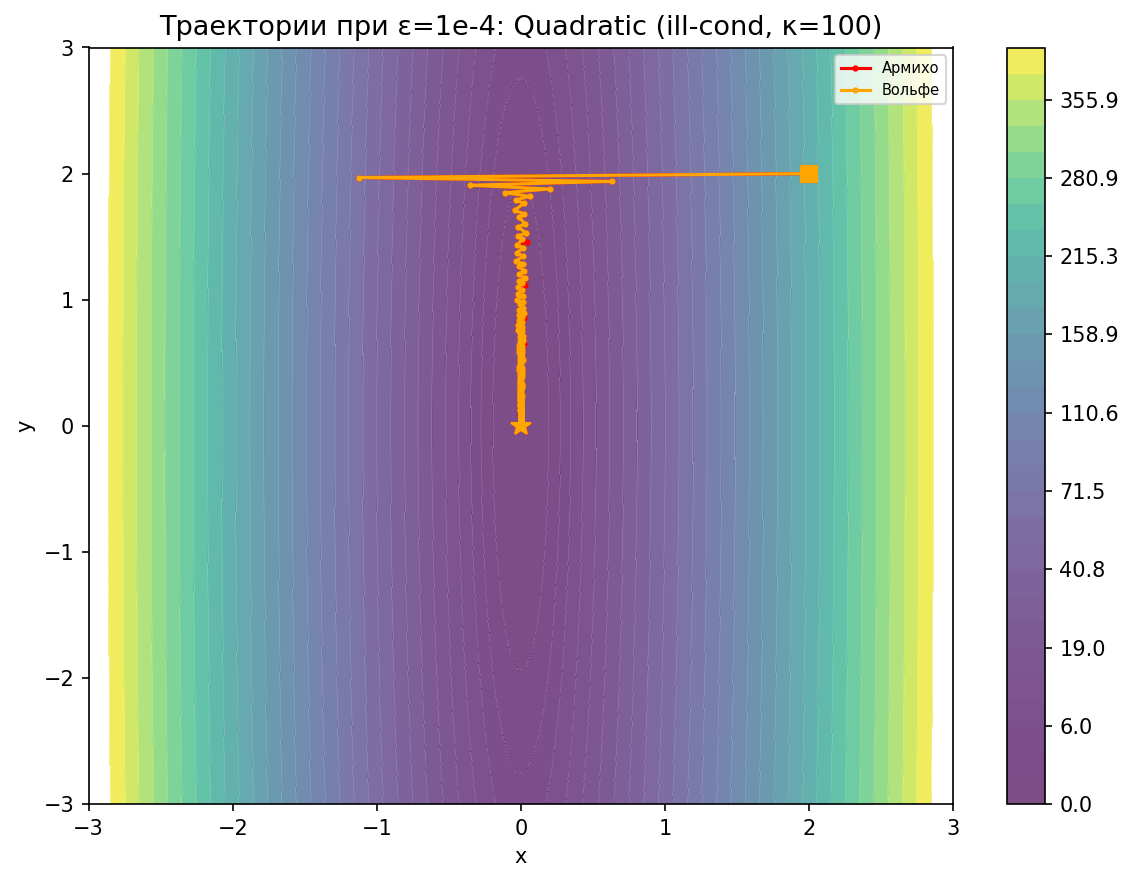
\includegraphics[width=\textwidth]{results/plots/fig_traj_linesearch_ill.png}
        \caption{Плохо обусловленная ($\kappa=100$)}
    \end{subfigure}
    \caption{Траектории методов Армихо и Вольфе при $\eps=10^{-4}$.
    Слева: оба метода за одну итерацию.
    Справа: Вольфе (оранжевый) — три прямых прыжка, Армихо (красный) — сотни зигзагов.}
    \label{fig:traj_linesearch}
\end{figure}

% ─────────────────────────────────────────────────────────────
\subsection{Задание 5: Методы дробления шага на сложных функциях}
% ─────────────────────────────────────────────────────────────

Запуски из нескольких стартовых точек при $\eps=10^{-8}$.

\begin{table}[H]
\centering
\caption{Розенброк: Армихо и Вольфе из разных стартовых точек.}
\label{tab:complex5_ros}
\begin{tabular}{lccccc}
\toprule
Метод & $x_0$ & Итерации & $f$-вызовы & $\grad$-вызовы & $f(x^*)$ \\
\midrule
Армихо & $(-1.0,\; 1.0)$ & 1 & 4 & 2 & $1.25\times10^{-16}$ \\
Вольфе & $(-1.0,\; 1.0)$ & 1 & 4 & 4 & $1.25\times10^{-16}$ \\
Армихо & $(\phantom{-}0.5, -0.5)$ & 20491 & 223753 & 20492 & $6.22\times10^{-17}$ \\
Вольфе & $(\phantom{-}0.5, -0.5)$ & 20413 & 222948 & 222948 & $6.59\times10^{-17}$ \\
Армихо & $(-1.5,\; 2.0)$ & 23360 & 258673 & 23361 & $6.12\times10^{-17}$ \\
Вольфе & $(-1.5,\; 2.0)$ & 20388 & 223086 & 223086 & $6.29\times10^{-17}$ \\
\bottomrule
\end{tabular}
\end{table}

\begin{table}[H]
\centering
\caption{Химмельблау: Армихо и Вольфе из разных стартовых точек.}
\label{tab:complex5_him}
\begin{tabular}{lccccc}
\toprule
Метод & $x_0$ & Итерации & $f$-вызовы & $\grad$-вызовы & $x^*$ \\
\midrule
Армихо & $(0.0,\; 0.0)$ & 30 & 229 & 31 & $(3,2)$ \\
Вольфе & $(0.0,\; 0.0)$ & 28 & 214 & 214 & $(3,2)$ \\
Армихо & $(-3.0,\; 3.0)$ & 16 & 129 & 17 & $(-2.81,3.13)$ \\
Вольфе & $(-3.0,\; 3.0)$ & 16 & 129 & 129 & $(-2.81,3.13)$ \\
Армихо & $(\phantom{-}3.0, -1.0)$ & 53 & 424 & 54 & $(3.58,-1.85)$ \\
Вольфе & $(\phantom{-}3.0, -1.0)$ & 53 & 424 & 424 & $(3.58,-1.85)$ \\
\bottomrule
\end{tabular}
\end{table}

\noindent\textit{Данные в таблицах получены из результатов выполнения программы.}

\begin{figure}[H]
    \centering
    \begin{subfigure}[b]{0.48\textwidth}
        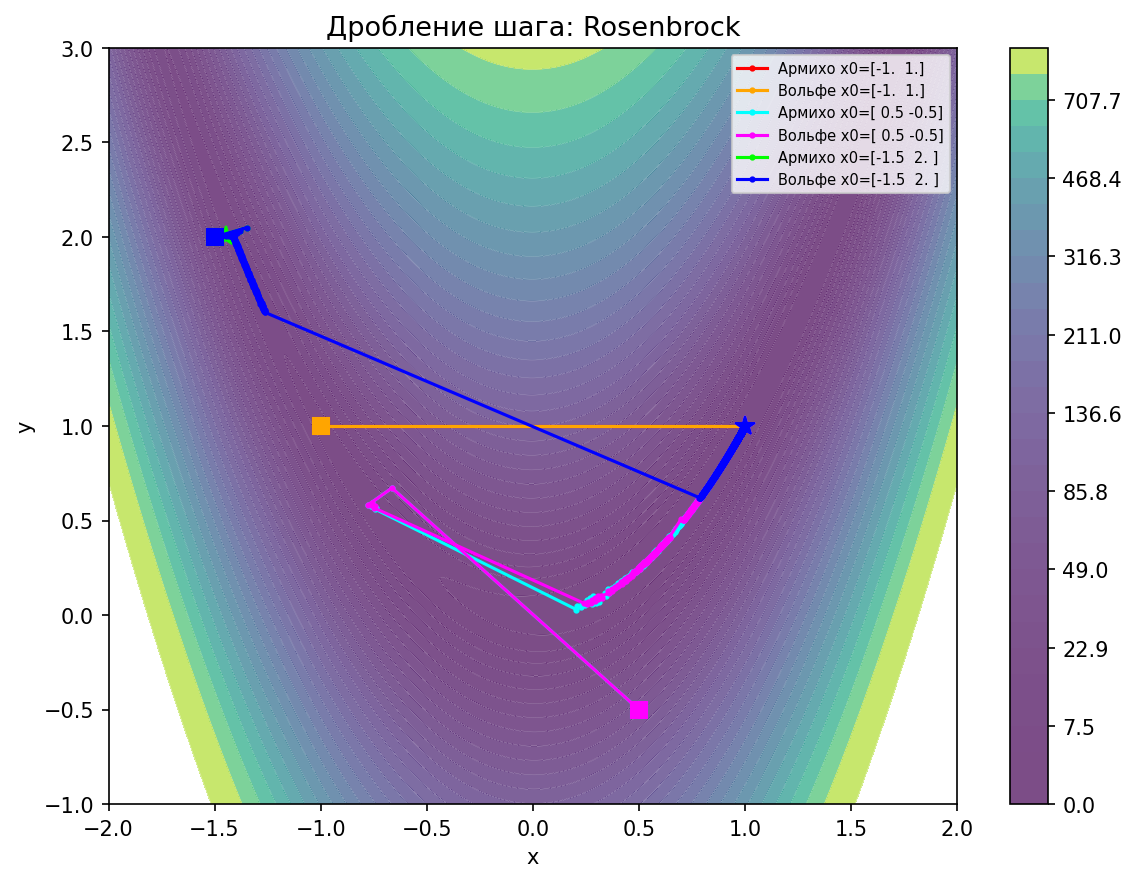
\includegraphics[width=\textwidth]{results/plots/fig_complex_linesearch_Ros.png}
        \caption{Розенброк}
    \end{subfigure}
    \hfill
    \begin{subfigure}[b]{0.48\textwidth}
        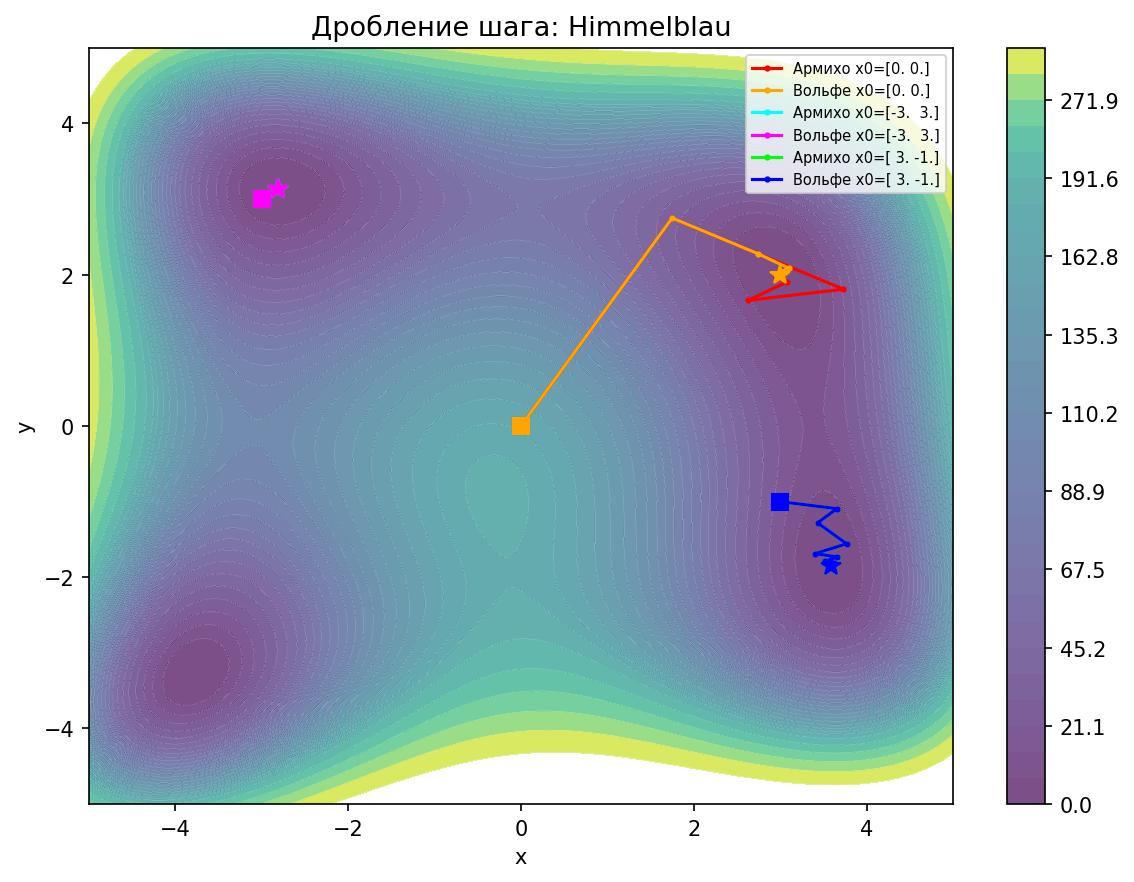
\includegraphics[width=\textwidth]{results/plots/fig_complex_linesearch_Him.png}
        \caption{Химмельблау}
    \end{subfigure}
    \caption{Траектории Армихо и Вольфе из нескольких стартовых точек.
    Розенброк: оба метода медленно ползут вдоль долины.
    Химмельблау: в зависимости от стартовой точки метод сходится к разным из четырёх минимумов.}
    \label{fig:complex5}
\end{figure}

% ─────────────────────────────────────────────────────────────
\subsection{Задание 6: Метод наискорейшего градиентного спуска}
% ─────────────────────────────────────────────────────────────

\subsubsection{Квадратичные функции — зависимость от точности}

% Auto-generated steepest-descent tables
\input{results/tables/Наискорейший_спуск__Quadratic__well_cond__κ_1_.tex}

\input{results/tables/Наискорейший_спуск__Quadratic__ill_cond__κ_100_.tex}

\paragraph{Вывод.}
На $\kappa=1$ метод сходится за \textbf{1 итерацию} — аналитическая формула
$\alpha^* = \norm{g}^2/(g^\top A g)$ даёт точный минимум.
На $\kappa=100$ траектория зигзагообразна: $g_{k+1} \perp g_k$, прогресс
вдоль длинной оси эллипса медленный.

\begin{figure}[H]
    \centering
    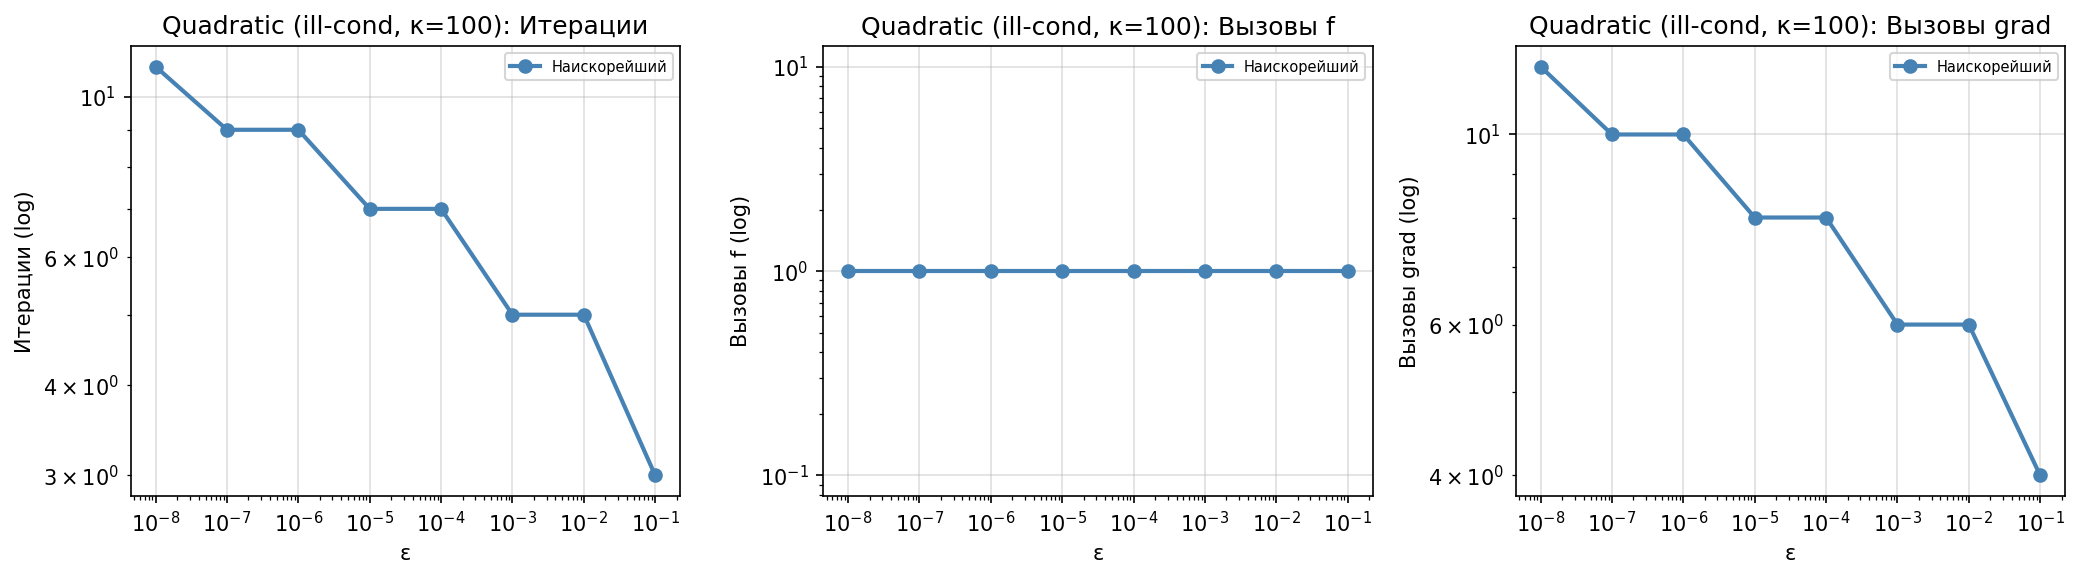
\includegraphics[width=\textwidth]{results/plots/fig_eps_steepest_ill.png}
    \caption{Зависимость числа итераций, вызовов $f$ и $\grad f$ от $\eps$
    для наискорейшего спуска на плохо обусловленной квадратике.}
    \label{fig:eps_steepest_ill}
\end{figure}

\begin{figure}[H]
    \centering
    \begin{subfigure}[b]{0.48\textwidth}
        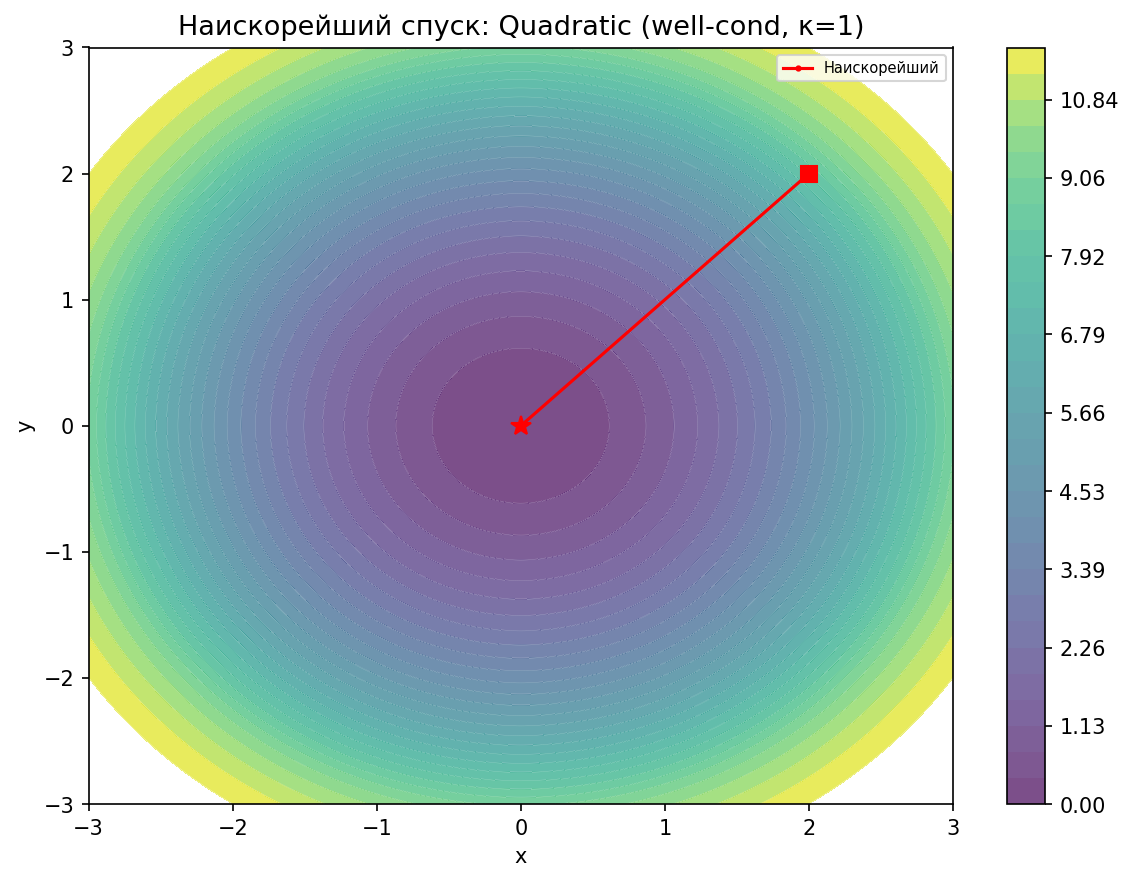
\includegraphics[width=\textwidth]{results/plots/fig_steepest_well.png}
        \caption{Хорошо обусловленная ($\kappa=1$)}
    \end{subfigure}
    \hfill
    \begin{subfigure}[b]{0.48\textwidth}
        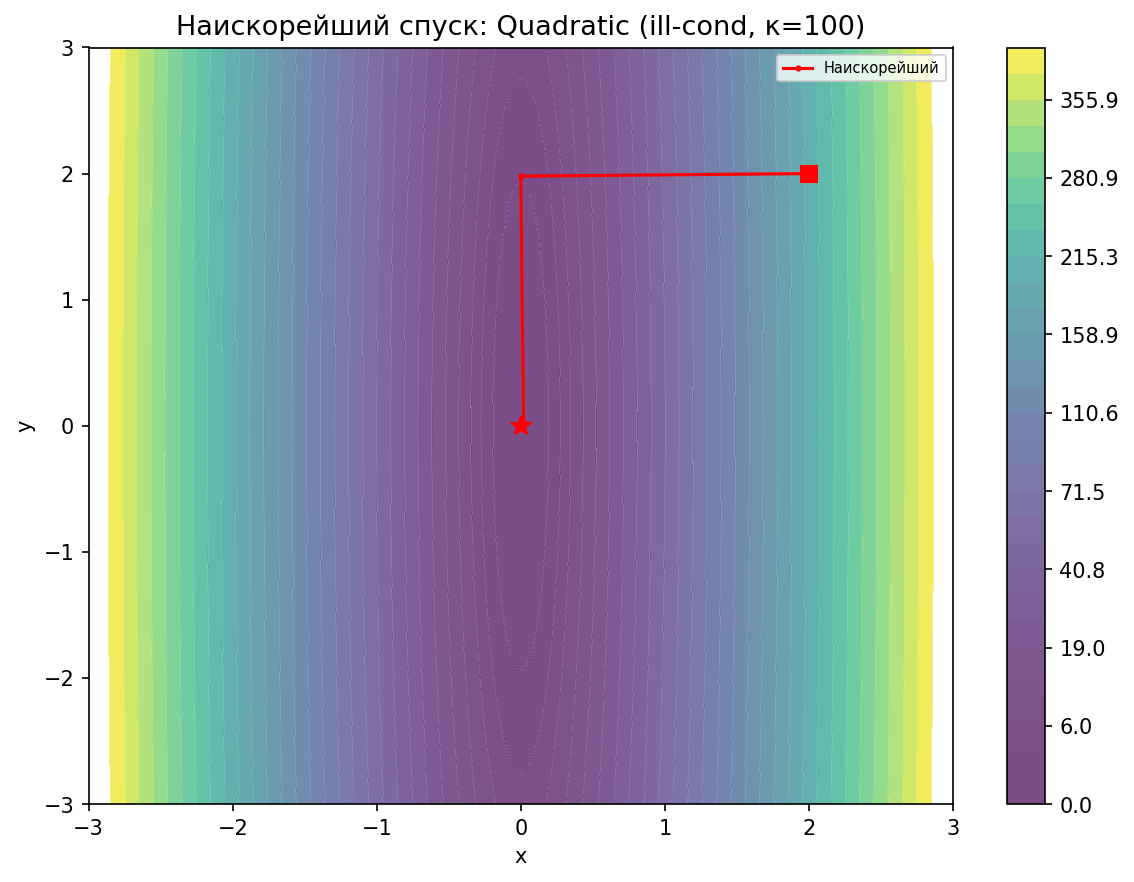
\includegraphics[width=\textwidth]{results/plots/fig_steepest_ill.png}
        \caption{Плохо обусловленная ($\kappa=100$)}
    \end{subfigure}
    \caption{Траектории наискорейшего спуска на квадратичных функциях.
    Слева: одна итерация до минимума.
    Справа: классические ортогональные зигзаги вдоль вытянутого эллипса.}
    \label{fig:steepest_quad}
\end{figure}

\subsubsection{Сложные функции}

\begin{table}[H]
\centering
\caption{Наискорейший спуск: Розенброк из разных стартовых точек.}
\label{tab:steepest_complex_ros}
\begin{tabular}{lcccc}
\toprule
$x_0$ & Итерации & $f$-вызовы & $\grad$-вызовы & $f(x^*)$ \\
\midrule
$(-1.0,\; 1.0)$ & 60 & 1242 & 61 & $1.24\times10^{-16}$ \\
$(0.5,\; -0.5)$ & 887 & 16168 & 888 & $1.19\times10^{-16}$ \\
\bottomrule
\end{tabular}
\end{table}

\begin{table}[H]
\centering
\caption{Наискорейший спуск: Химмельблау из разных стартовых точек.}
\label{tab:steepest_complex_him}
\begin{tabular}{lcccc}
\toprule
$x_0$ & Итерации & $f$-вызовы & $\grad$-вызовы & $x^*$ \\
\midrule
$(0.0,\; 0.0)$ & 29 & 533 & 30 & $(3,2)$ \\
$(-3.0,\; 3.0)$ & 37 & 717 & 38 & $(-2.81,3.13)$ \\
\bottomrule
\end{tabular}
\end{table}

\begin{figure}[H]
    \centering
    \begin{subfigure}[b]{0.48\textwidth}
        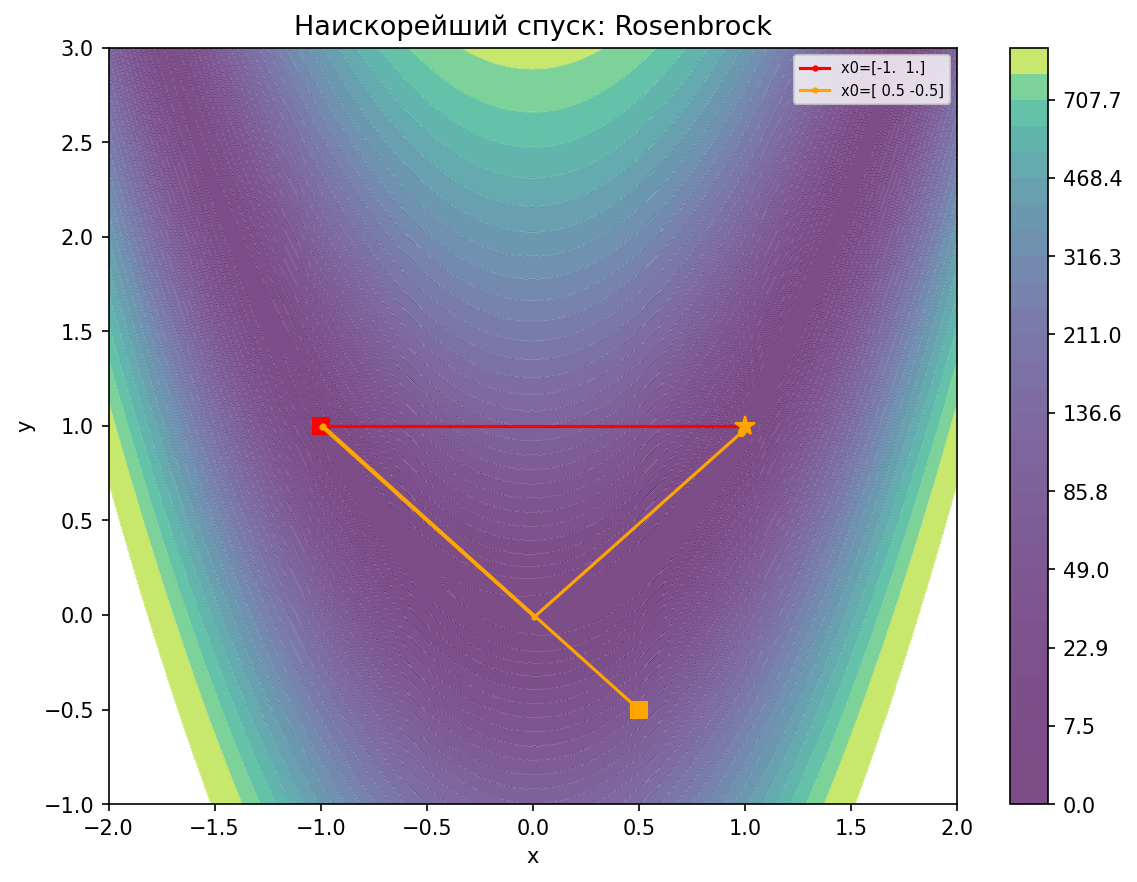
\includegraphics[width=\textwidth]{results/plots/fig_steepest_complex_Ros.png}
        \caption{Розенброк}
    \end{subfigure}
    \hfill
    \begin{subfigure}[b]{0.48\textwidth}
        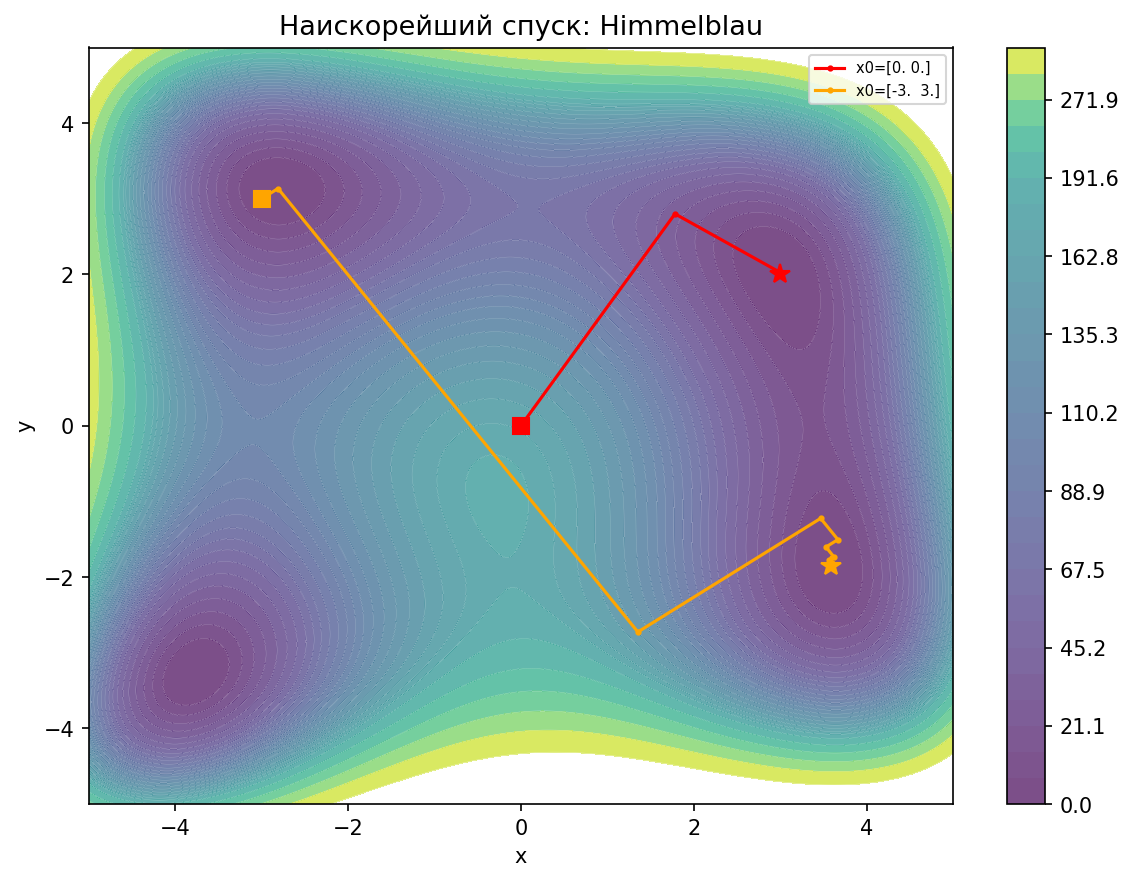
\includegraphics[width=\textwidth]{results/plots/fig_steepest_complex_Him.png}
        \caption{Химмельблау}
    \end{subfigure}
    \caption{Траектории наискорейшего спуска из нескольких стартовых точек.
    Розенброк: точная минимизация по шагу не помогает преодолеть узкую долину —
    метод всё равно медленно ползёт.
    Химмельблау: результат зависит от стартовой точки.}
    \label{fig:steepest_complex}
\end{figure}

% ═════════════════════════════════════════════════════════════
\section{Общие выводы}
% ═════════════════════════════════════════════════════════════

\begin{enumerate}
    \item \textbf{Постоянный шаг.}
    Прост в реализации, но требует ручного подбора $\alpha \in (0, 2/L)$.
    Для хорошо обусловленных задач оптимальный шаг вычислим теоретически.
    На плохо обусловленных ($\kappa \gg 1$) число итераций пропорционально $\kappa$.
    На сложных функциях большие шаги приводят к расходимости из-за взрыва градиента.

    \item \textbf{Число обусловленности $\kappa$} — главный параметр.
    Постоянный шаг: $k \sim \mathcal{O}(\kappa)$.
    Наискорейший спуск на квадратике: $k \sim \mathcal{O}(\kappa)$ из-за
    зигзагообразности.
    Методы с условиями Вольфе на квадратике: $k \sim \mathcal{O}(1)$ (!) за счёт
    выбора шага близкого к оптимальному.

    \item \textbf{Армихо vs Вольфе.}
    Вольфе выигрывает в разы на плохо обусловленных задачах:
    3 итерации против 869 при $\kappa=100$.
    На хорошо обусловленных задачах разница незначительна.
    Армихо проще в реализации, Вольфе надёжнее в сложных случаях.

    \item \textbf{Наискорейший спуск.}
    На квадратиках с $\kappa=1$ — оптимален (1 итерация).
    На квадратиках с $\kappa=100$ — медленнее Вольфе: зигзагообразная траектория
    из-за ортогональности последовательных градиентов.
    На сложных функциях без аналитической формулы $\alpha^*$ требует численной
    одномерной минимизации, что увеличивает число вызовов $f$.

    \item \textbf{Многоэкстремальные функции.}
    Градиентные методы первого порядка не гарантируют глобального минимума.
    Результат принципиально зависит от стартовой точки.
    Для борьбы с этим используют многократные перезапуски из разных точек.
\end{enumerate}

\end{document}